\section{Process\-Monitor Class Reference}
\label{classProcessMonitor}\index{ProcessMonitor@{ProcessMonitor}}
Inheritance diagram for Process\-Monitor:\begin{figure}[H]
\begin{center}
\leavevmode
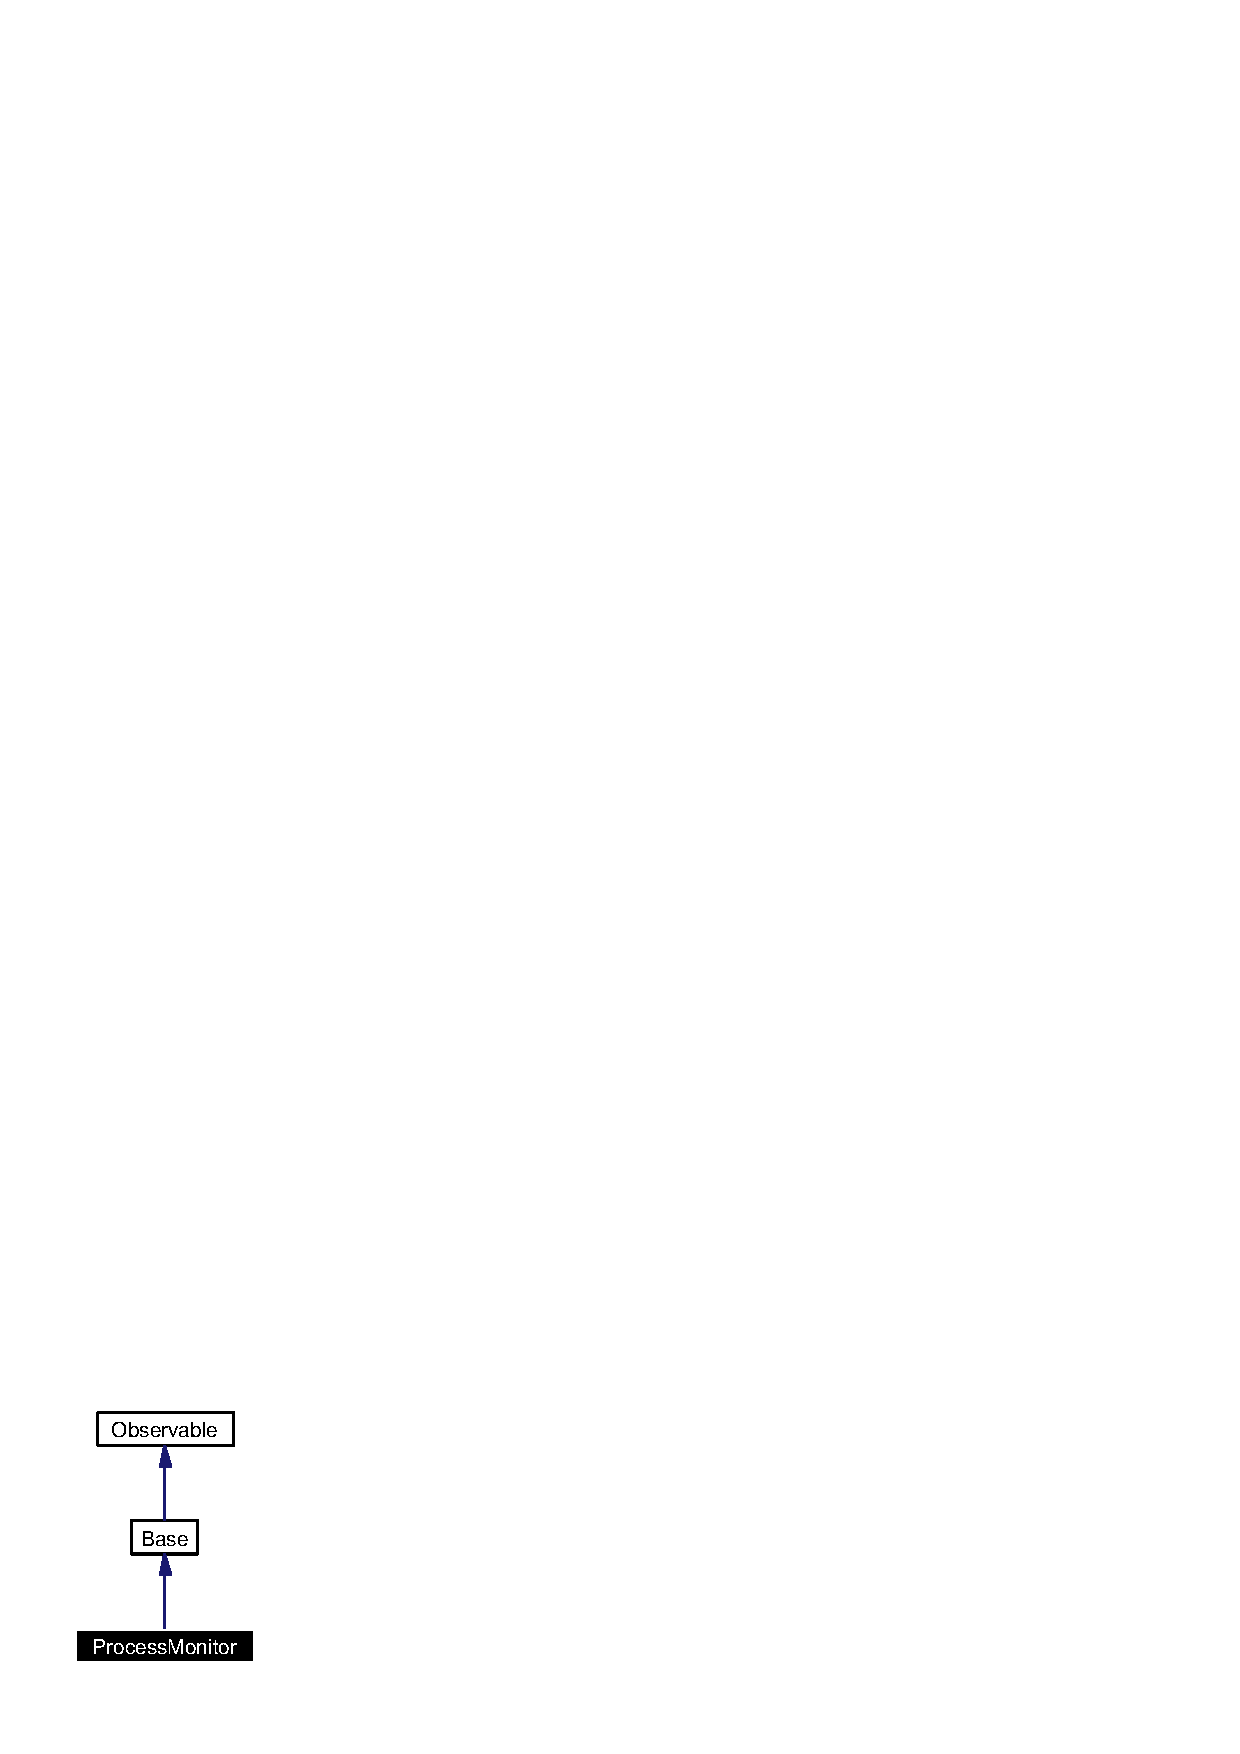
\includegraphics[width=61pt]{classProcessMonitor__inherit__graph}
\end{center}
\end{figure}
Collaboration diagram for Process\-Monitor:\begin{figure}[H]
\begin{center}
\leavevmode
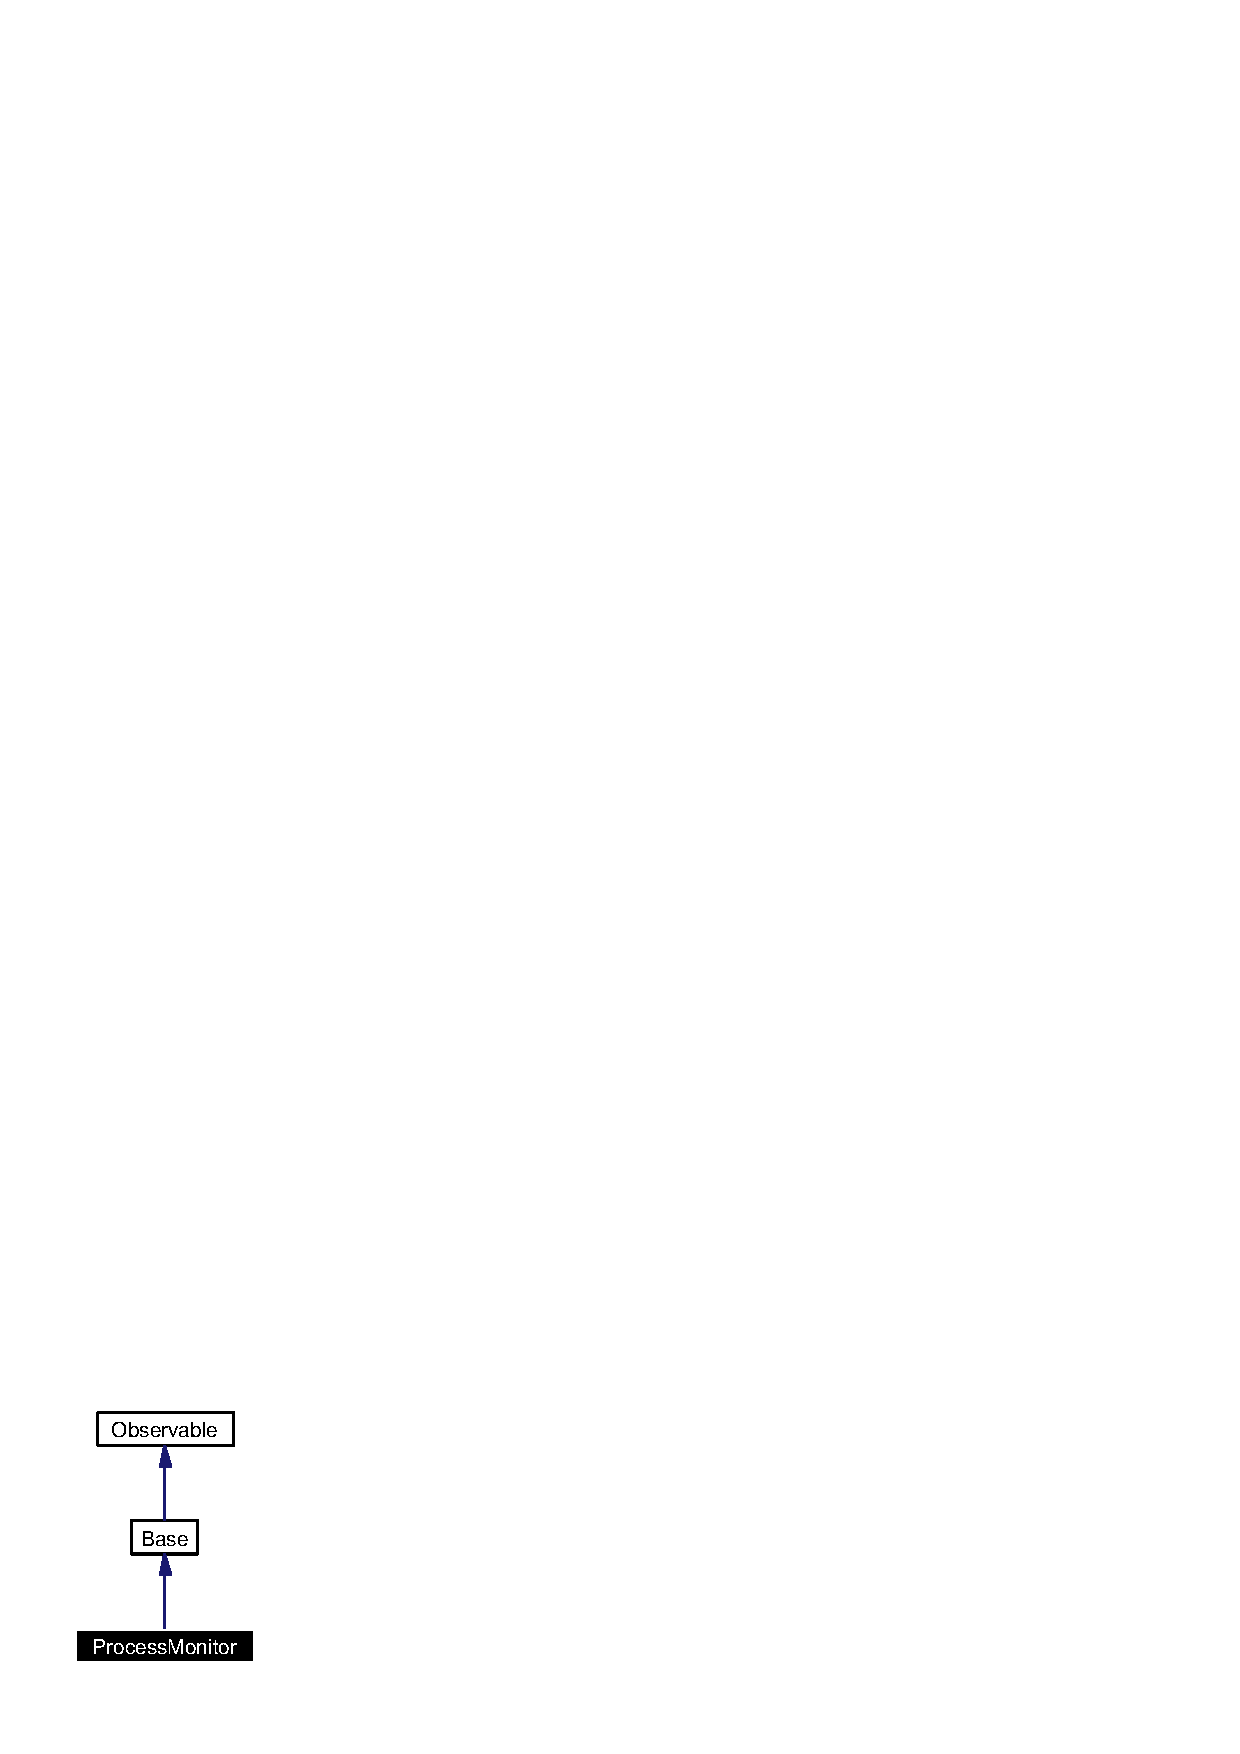
\includegraphics[width=61pt]{classProcessMonitor__coll__graph}
\end{center}
\end{figure}
\subsection*{Public Member Functions}
\begin{CompactItemize}
\item 
{\bf monitor\_\-stats} ()\label{classProcessMonitor_a0}

\item 
{\bf update\_\-instance\_\-status} (\$iid, \$status)\label{classProcessMonitor_a1}

\item 
{\bf update\_\-instance\_\-activity\_\-status} (\$iid, \$activity\-Id, \$status)\label{classProcessMonitor_a2}

\item 
{\bf remove\_\-instance} (\$iid)\label{classProcessMonitor_a3}

\item 
{\bf remove\_\-aborted} ()\label{classProcessMonitor_a4}

\item 
{\bf remove\_\-all} (\$p\-Id)\label{classProcessMonitor_a5}

\item 
{\bf monitor\_\-list\_\-processes} (\$offset, \$max\-Records, \$sort\_\-mode, \$find, \$where='')\label{classProcessMonitor_a6}

\item 
{\bf monitor\_\-list\_\-activities} (\$offset, \$max\-Records, \$sort\_\-mode, \$find, \$where='')\label{classProcessMonitor_a7}

\item 
{\bf monitor\_\-list\_\-instances} (\$offset, \$max\-Records, \$sort\_\-mode, \$find, \$where='', \$wherevars)\label{classProcessMonitor_a8}

\item 
{\bf monitor\_\-list\_\-all\_\-processes} (\$sort\_\-mode)\label{classProcessMonitor_a9}

\item 
{\bf monitor\_\-list\_\-statuses} ()\label{classProcessMonitor_a10}

\item 
{\bf monitor\_\-list\_\-users} ()\label{classProcessMonitor_a11}

\item 
{\bf monitor\_\-list\_\-wi\_\-users} ()\label{classProcessMonitor_a12}

\item 
{\bf monitor\_\-list\_\-owners} ()\label{classProcessMonitor_a13}

\item 
{\bf monitor\_\-list\_\-activity\_\-types} ()\label{classProcessMonitor_a14}

\item 
{\bf monitor\_\-get\_\-workitem} (\$item\-Id)\label{classProcessMonitor_a15}

\item 
{\bf monitor\_\-list\_\-workitems} (\$offset, \$max\-Records, \$sort\_\-mode, \$find, \$where='', \$wherevars=array())\label{classProcessMonitor_a16}

\end{CompactItemize}


\subsection{Detailed Description}
This class provides methods for use in typical monitoring scripts 



Definition at line 8 of file Process\-Monitor.php.

The documentation for this class was generated from the following file:\begin{CompactItemize}
\item 
Process\-Monitor.php\end{CompactItemize}
